\section{进程相似性分析}

使用\perflow{}实现进程相似性分析的分析任务,在NPB基准测试程序上进行测试。测试结果如下:

\begin{figure}[!h]
  \setcounter{subfigure}{0}
  \centering
  % \includegraphics[width=0.9\textwidth]{}
  \subfigure[BT]{
    \centering
    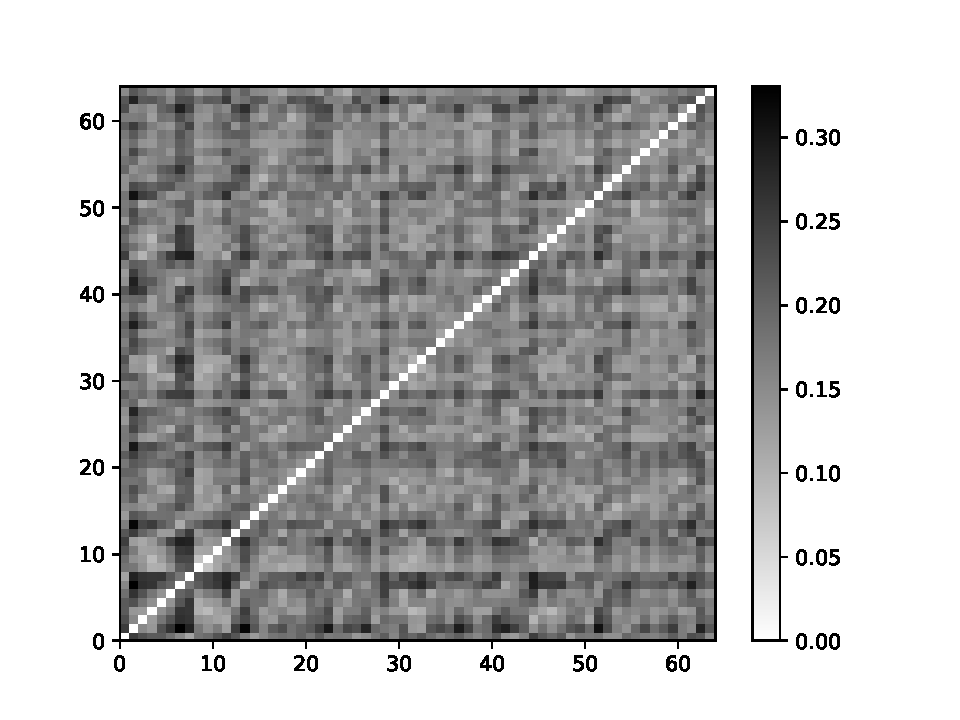
\includegraphics[width=0.3\textwidth]{procs_similarity/bt.B.pdf}
  }
  \subfigure[CG]{
    \centering
    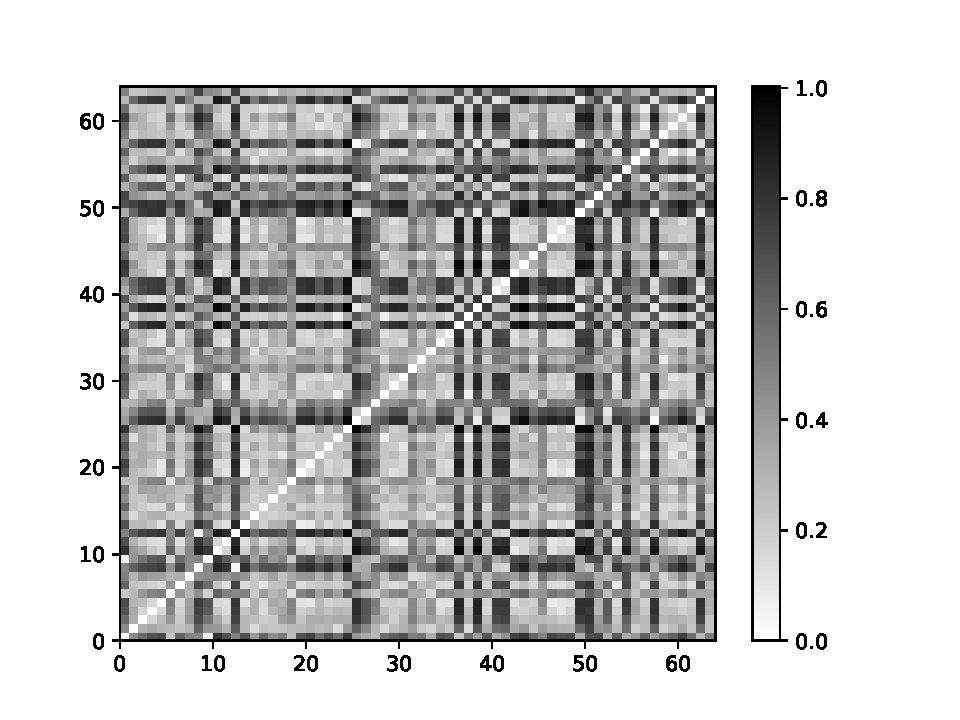
\includegraphics[width=0.3\textwidth]{procs_similarity/cg.B.pdf}
  }
  \subfigure[DT]{
    \centering
    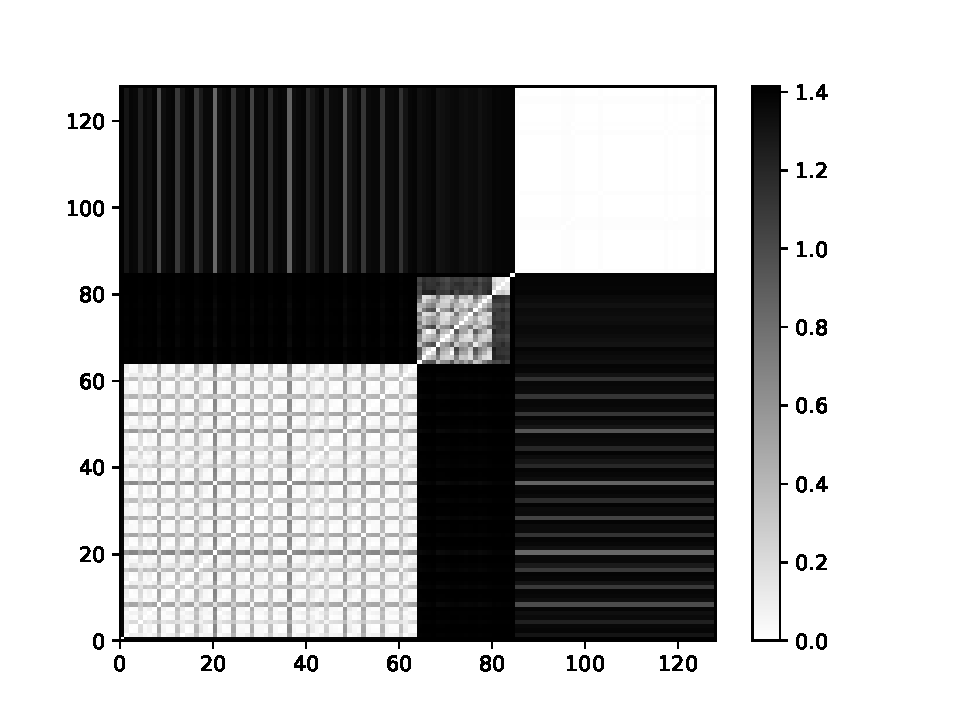
\includegraphics[width=0.3\textwidth]{procs_similarity/dt.C.pdf}
  }
  \subfigure[EP]{
    \centering
    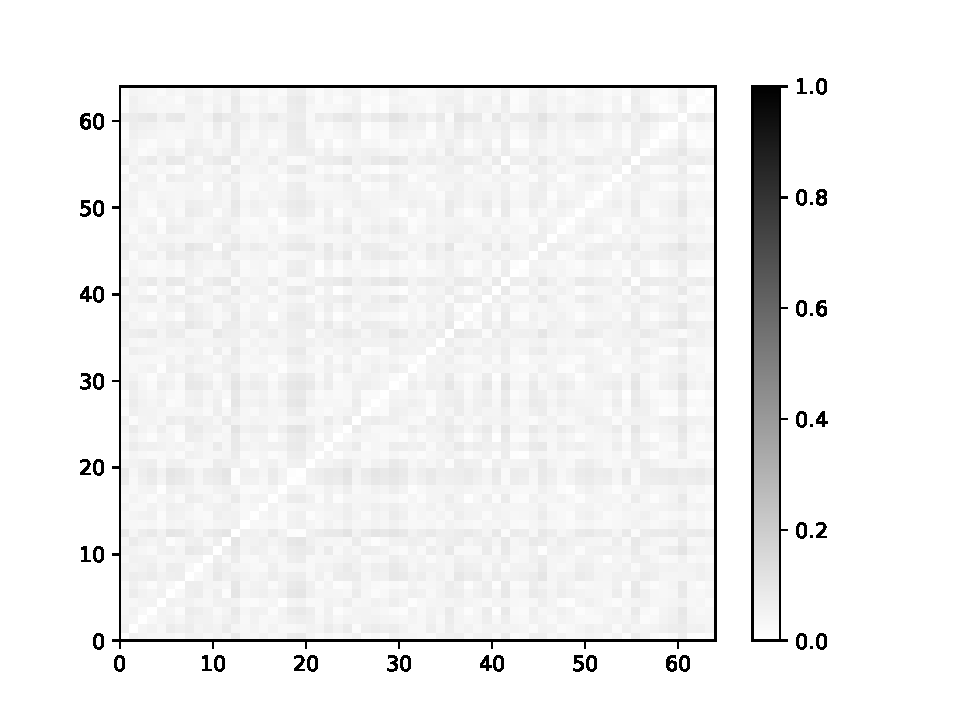
\includegraphics[width=0.3\textwidth]{procs_similarity/ep.C.pdf}
  }
  \subfigure[FT]{
    \centering
    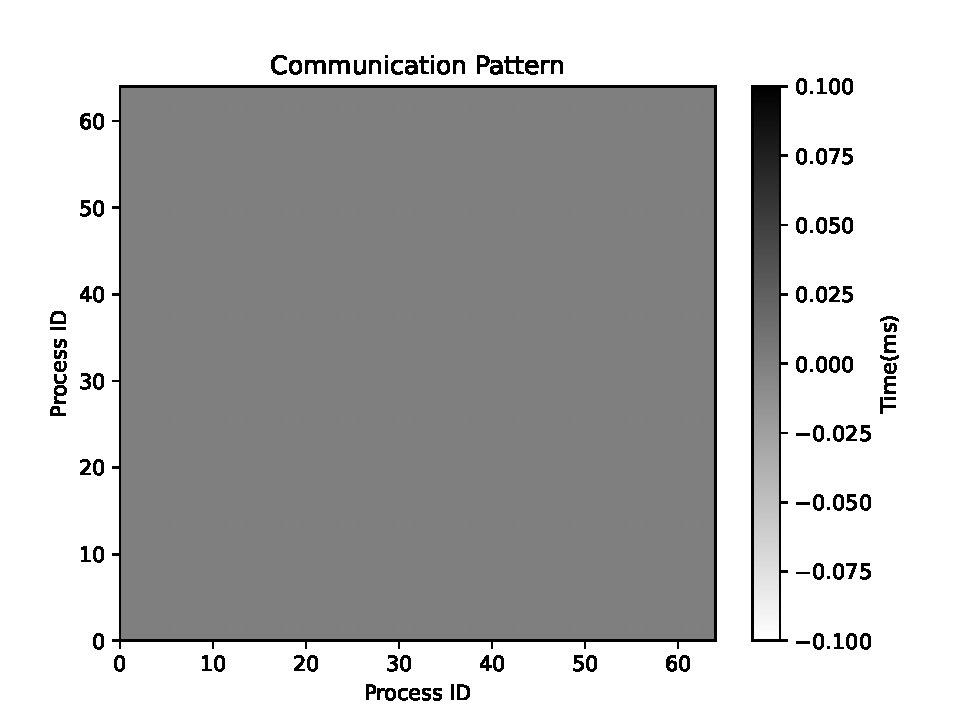
\includegraphics[width=0.3\textwidth]{procs_similarity/ft.B.pdf}
  }
  \subfigure[IS]{
    \centering
    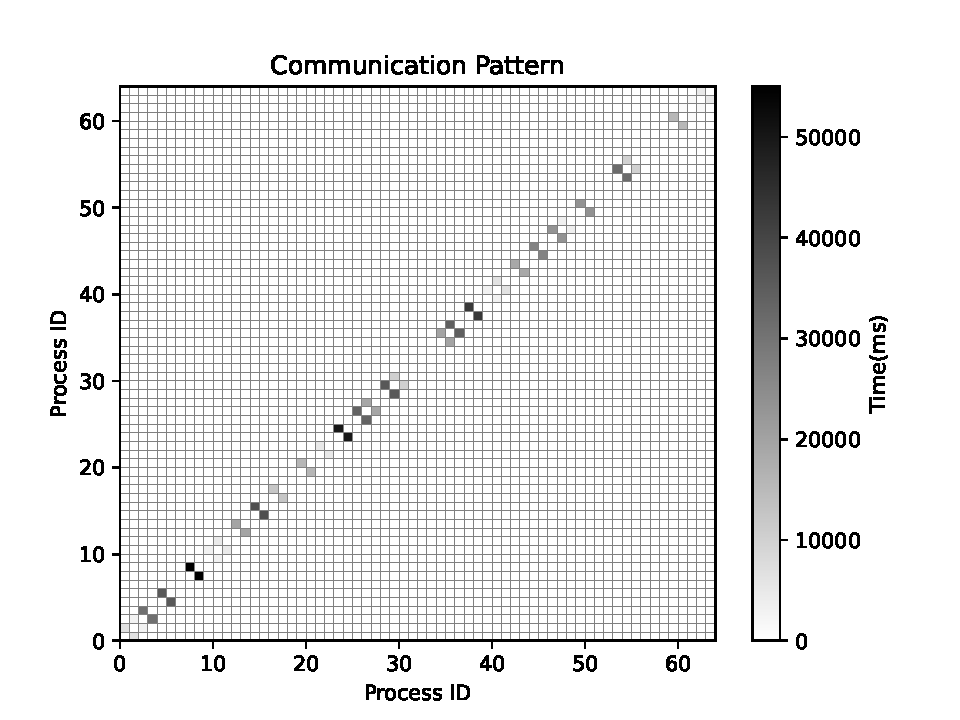
\includegraphics[width=0.3\textwidth]{procs_similarity/is.C.pdf}
  }
  \subfigure[LU]{
    \centering
    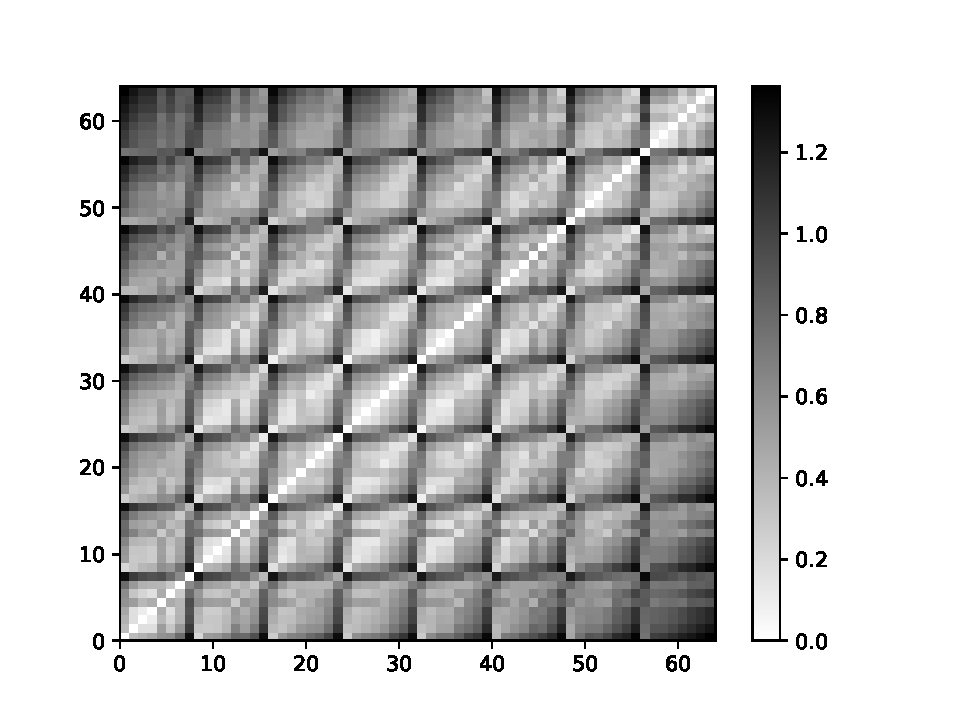
\includegraphics[width=0.3\textwidth]{procs_similarity/lu.B.pdf}
  }
  \subfigure[SP]{
    \centering
    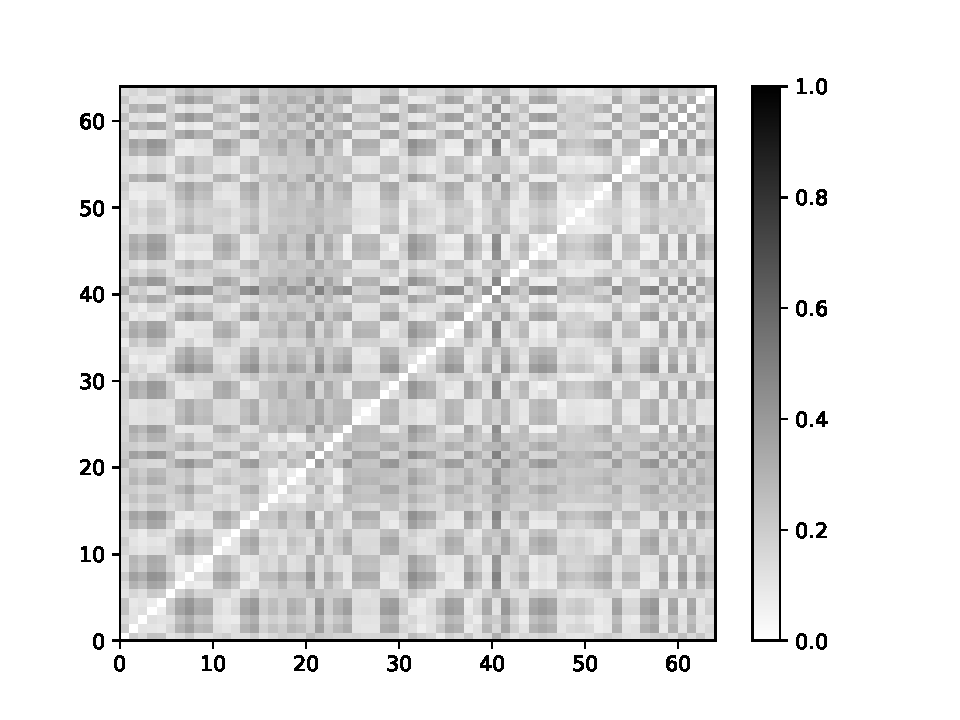
\includegraphics[width=0.3\textwidth]{procs_similarity/sp.B.pdf}
  }
  \subfigure[MG]{
    \centering
    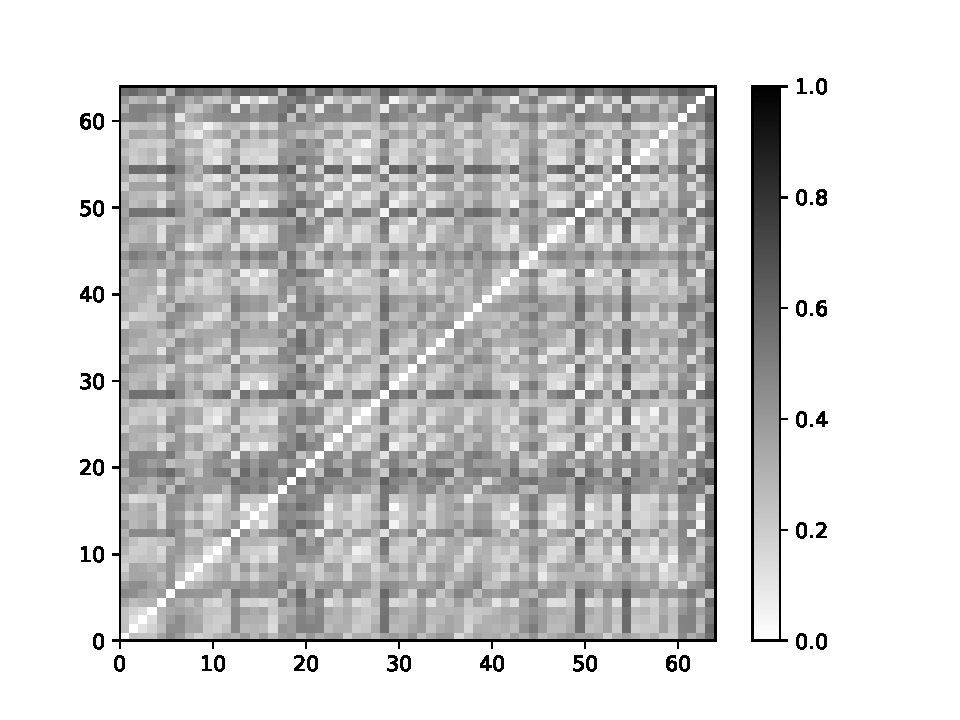
\includegraphics[width=0.3\textwidth]{procs_similarity/mg.C.pdf}
  }
\end{figure}

在SWEEP3D和LULESH上进行测试。测试结果如下:

\begin{figure}[!h]
  \centering
  \subfigure[SWEEP3D]{
    \centering
    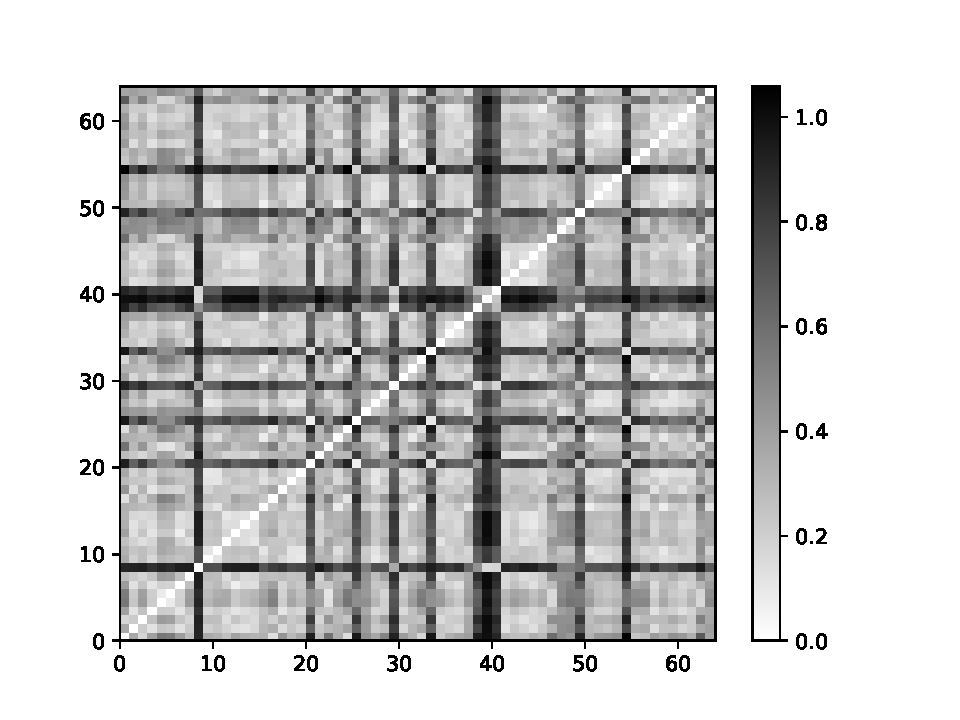
\includegraphics[width=0.4\textwidth]{procs_similarity/sweep3d.pdf}
  }
  \subfigure[LULESH]{
    \centering
    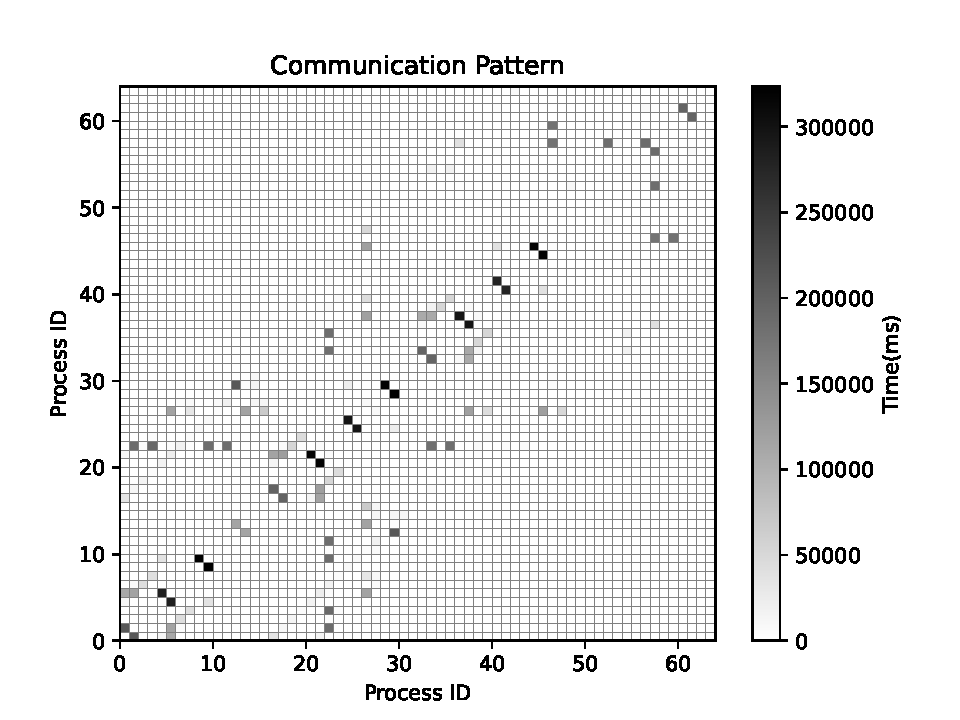
\includegraphics[width=0.4\textwidth]{procs_similarity/lulesh.pdf}
  }
\end{figure}

在HPL(High Performance Linpack)和HPCG上进行测试。测试结果如下:

\begin{figure}[!h]
  \setcounter{subfigure}{0}
  \centering
  \subfigure[HPL]{
    \centering
    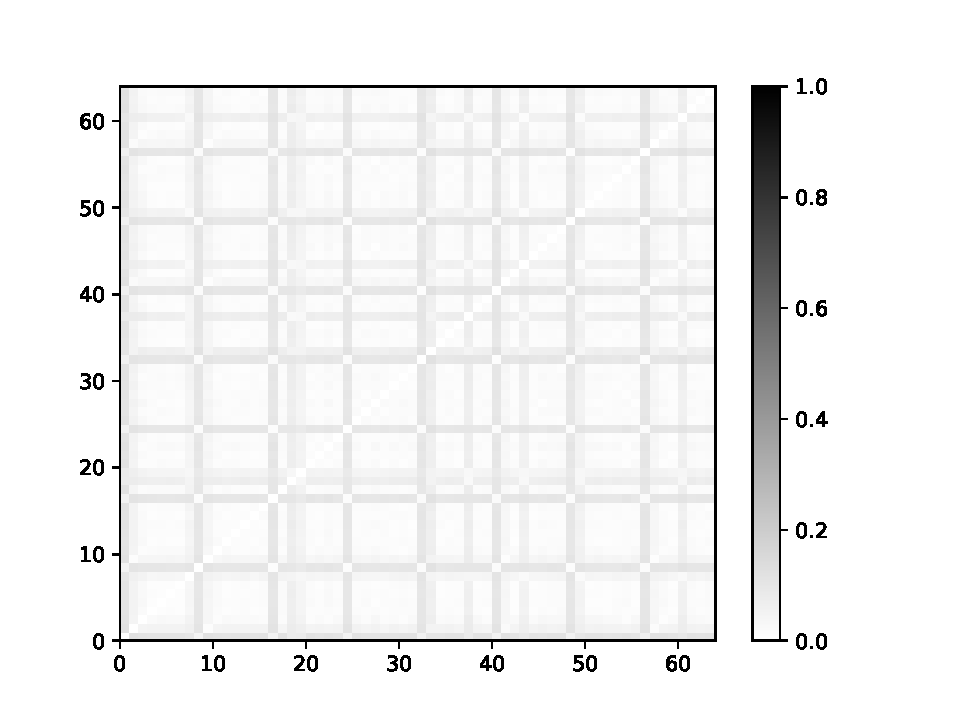
\includegraphics[width=0.4\textwidth]{procs_similarity/hpl.pdf}
  }
  \subfigure[HPCG]{
    \centering
    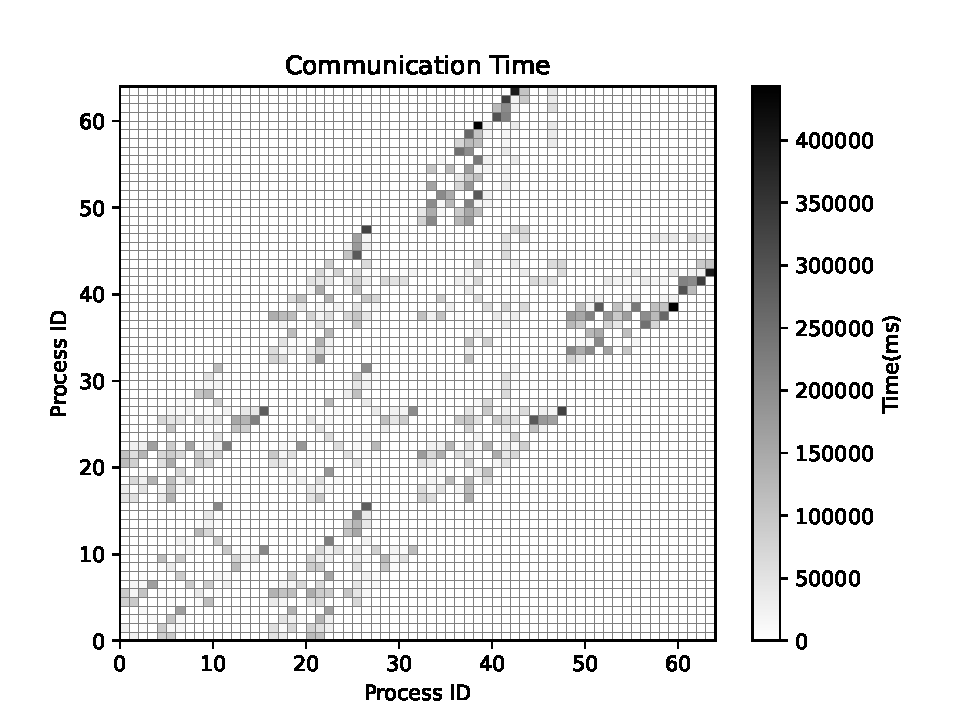
\includegraphics[width=0.4\textwidth]{procs_similarity/hpcg.pdf}
  }
\end{figure}


在LAMMPS和QE上进行测试。测试结果如下:

\begin{figure}[!h]
  \setcounter{subfigure}{0}
  \centering
  \subfigure[LAMMPS]{
    \centering
    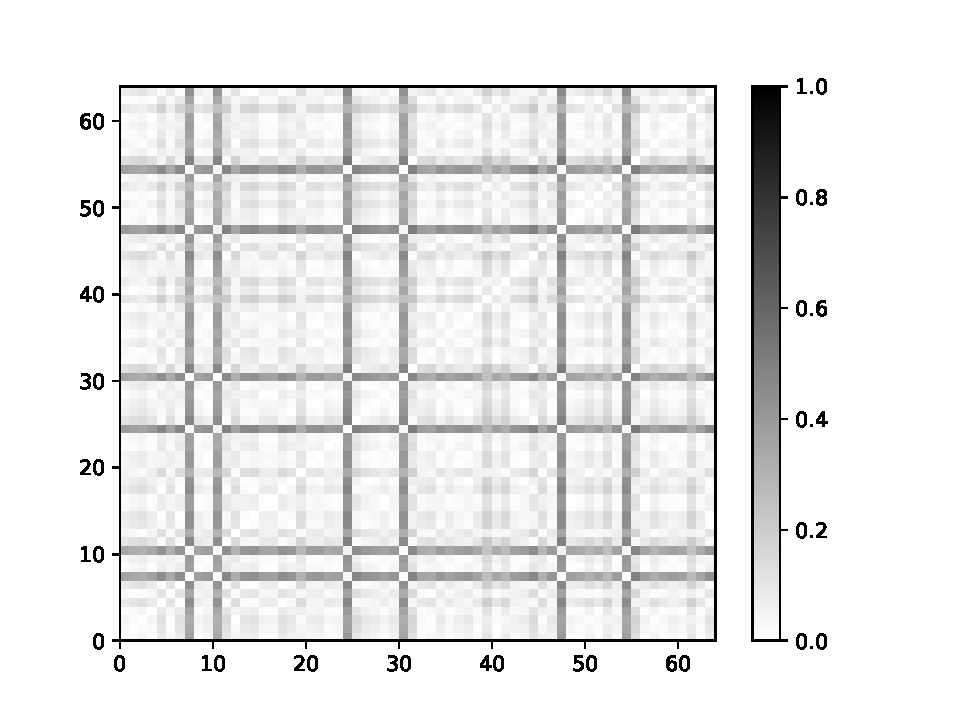
\includegraphics[width=0.3\textwidth]{procs_similarity/lammps.pdf}
  }
  \subfigure[QE npool=16]{
    \centering
    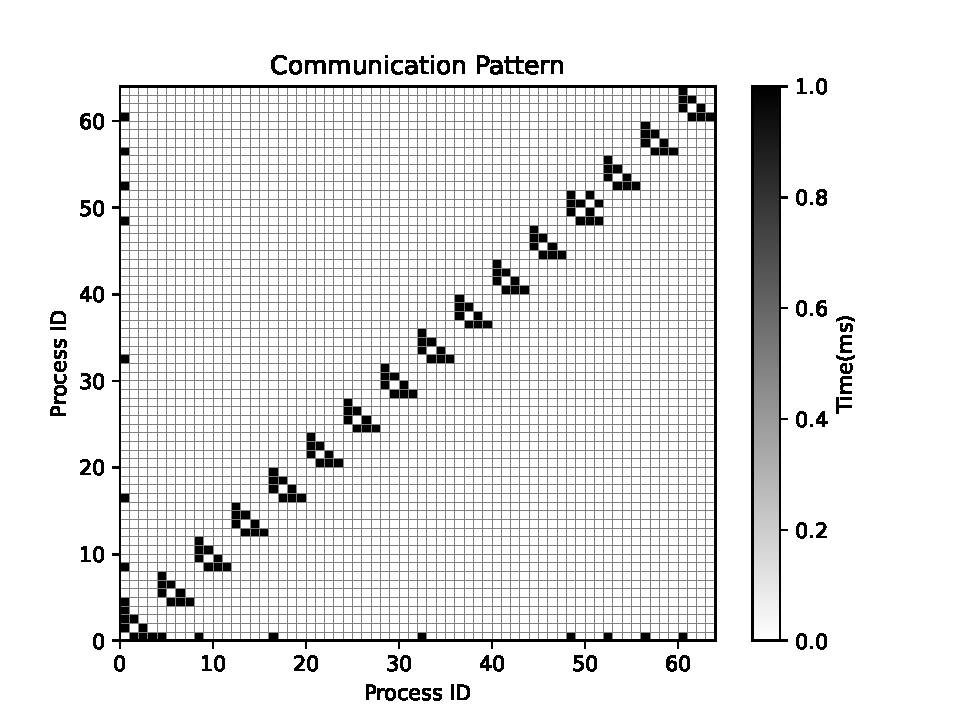
\includegraphics[width=0.3\textwidth]{procs_similarity/pw.x-npool16.pdf}
  }
  \subfigure[QE npool=8]{
    \centering
    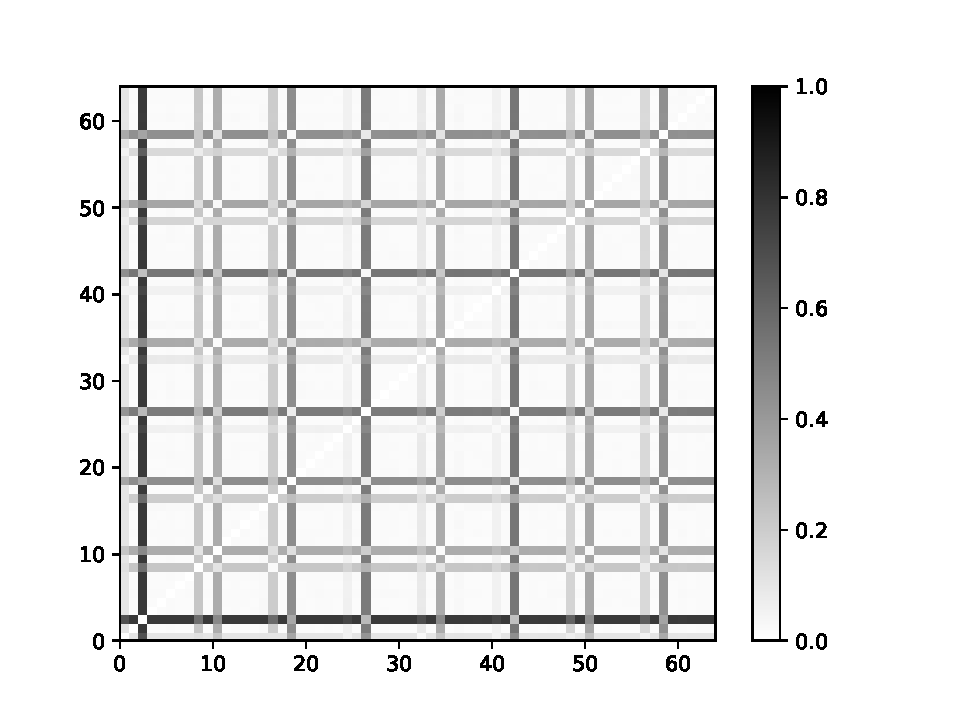
\includegraphics[width=0.3\textwidth]{procs_similarity/pw.x-npool8.pdf}
  }
\end{figure}